%!TEX root = paper.tex
\subsection{General settings}
I use a Bertrand pricing game model to characterize the fiscal competition between
Chinese city governments. In this model, each firm
signs a contract of producing
a given amount of output at given prices with the buyers on the global market.\footnote{
    The ``firms'' defined in this paper
    are private firms (Chinese private firms and foreign firms). State-owned firms are excluded
    from analysis since the goal of state-owned firms cannot be simply characterized
    as profit maximization,
    and they don't have absolute freedom to choose their locations.}
With fixed output levels, each firm makes a short list of potential cities for building
its factories,
then the firm solves the production cost minimization problem and builds its
factories in the city that is in its choice set and has the lowest production cost.\footnote{
    The assumption is valid since an individual firm has only limited information
    and political resources, so it can only deal with a limited number of city governments.}

The production cost of each firm is composed of four parts in the model:
\bnt
\item Capital cost: I assume that the price of capital is the same across the country.
\item Labor cost: I assume that
each city has a wage level determined by the local labor market.
An individual firm is just a price-taker in the labor market.
\item Land cost: The industrial land price is completely controlled by the city government,
and the city government makes a special land price offer for
each firm considering landing in its jurisdiction.
\item Other costs: all other costs (dependent on both firm and city characteristics)
are included in the error term of the model,
the distribution of which is common knowledge for all city governments.
\ent

The city governments maximize their expected fiscal revenue by
attracting firms to land in their jurisdictions. The term
``fiscal revenue'' here is most broadly defined, which includes
but is not limited to tax revenue,
promotion of local businesses and housing market, political benefits, etc., i.e.
all the potential benefits generated by landing firms.

The channel by which city governments attract firms is to provide
special industrial land price offers to the firms.
Since the output level of each firm is common knowledge for all city governments
in the firm's choice set, the city governments can adjust the production cost of a firm
by changing the land price offered to the firm.
This will change the probability
of the firm to land in this city as well as the expected fiscal
revenue for the city government to attract the firm.
And to determine the land price, a city government must consider the land prices
offered by other city governments, since the other city governments' price choices
will also impact the probability of the city getting the firm
as well as the city's expected fiscal revenue.
Thus, I use a Bertrand pricing game model to characterize the
strategic interaction of city governments
when they make the land offers.
At the Nash equilibrium of this game, each city government
has no incentive to change its land offer since the land price at the equilibrium
has already maximized its expected fiscal revenue given other cities' land offers in the
equilibrium strategy profile.

The main structure of the model implied in the discussion above can be described
using \Cref{fig:model structure} below:
\begin{figure}[H]
    \centering
    \caption{Main structure of the model}
    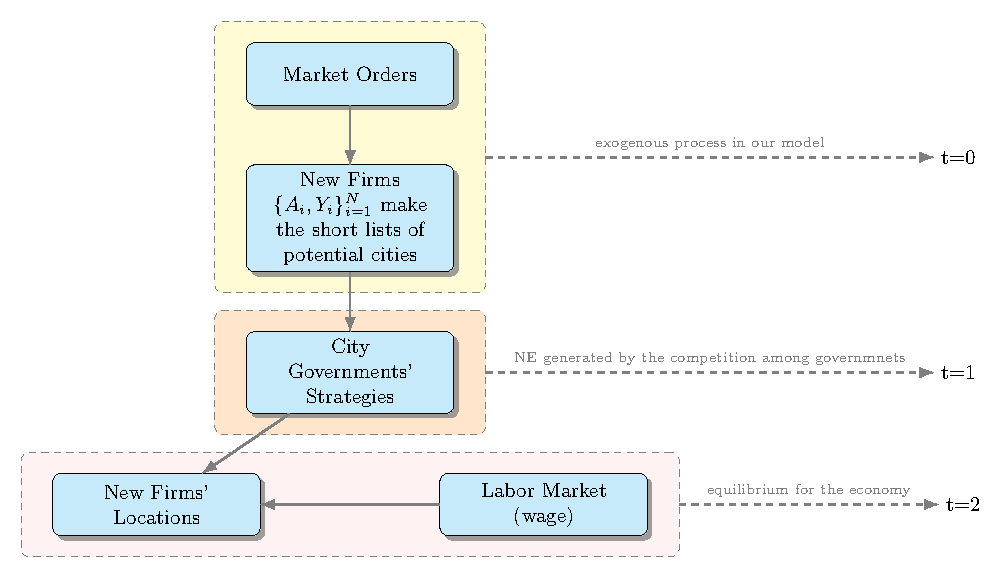
\includegraphics[scale=0.9]{\graphs/timing/timing.pdf}
    \label{fig:model structure}
    \fnote{Notes: The figure presents the main structure and timing assumptions of the model.
        Solid arrows represent causal channels in the model.
        I use the productivity of firm $i$, $A_i$
        and the output level $Y_i$ to characterize firm $i$ in this figure.}
\end{figure}
Next, I describe the cost minimization and location choice problems faced by firms,
then I write down the expected fiscal revenue maximization problem faced by city governments
as well as the Bertrand pricing game between city governments.
Finally, I define the pure strategy Nash equilibrium (NE) in this game
and prove the uniqueness of pure NE.

\subsection{Firms}
I index new private firms by $ i = 1,~\dots,~N$;
cities and city governments by $k = 1,~\dots,~M$.
Each firm $i$ is characterized by its output level $Y_i$
as well as its production function $F_i$, which is a mixture of Cobb-Douglas
and Leontief technology:
$$
    F_{i}(K, L, T)=\min \left\{A_{i} K^{\alpha} L^{1-\alpha}, g_{i}(T)\right\}.
$$

Here $A_i$ is the productivity of firm $i$,
$K$ is the amount of capital the firm uses in production,
$L$ is the number of workers,
$T$ is the area of industrial the firm $i$ uses,
and $g_i(\cdot)$ is a strictly increasing function which reflects that land is
a special input, which restricts the maximum output level of capital and labor.
Notice that in this production function, capital and labor can substitute each other, and
the land is the pure complement for capital and labor.
I also make the no-waste assumption, i.e., firms make full use of the lands.

Given the output level $Y_i$ firm $i$ needs to produce,
it chooses a city $k$ in its choice set
$\mathbf{C}_{i}$ (the short list of candidate cities) to build the factory,
as well as the amount of capital input $K_i$ per year,
number of workers $L_i$ and the area of industrial land $T_i$.
Thus, firm $i$ solves the following cost minimization problem:
\begin{equation}
    \begin{aligned}
         & \min _{k \in \mathbf{C}_{i}, K_{i}, L_{i}, T_{i}}
        \left\{r K_{i}+w_{k} L_{i}+\frac{p_{i k}}{m} T_{i}-\varepsilon_{i k}\right\}     \\
         & \text { s.t. } Y_{i}=\min \left\{A_{i} K_{i}^{\alpha} L_{i}^{1-\alpha}, g_{i}
        \left(T_{i}\right)\right\},
    \end{aligned}
    \label{firm_minimization1}
\end{equation}
where $r$ is the price of capital, which is assumed to be a constant in the whole country;
$w_k$ is the wage level in city $k$, which corresponds to the setting that
firm $i$ is just a price taker in the labor market;
$p_{ik}$ is the industrial land price city government $k$
offers to firm $i$; $m$ is the term of land lease.\footnote{
    I drop the subscript of m since
    the terms of the land lease in my data set are all 50 years.}
I divide $p_{ik}$ by $m$ so that the time scales for all variables are unified to a year,
and the firm is minimizing the production cost per year.
The term $\varepsilon_{ik}$ in the production
cost is an error term, which is assumed to have
type \RomanNumeralCaps{1} extreme value distribution with scale parameter $\sigma$.
It represents all other unobserved costs and benefits for the firm $i$ to
produce in the city $k$.

Furthermore, the price of one unit of product is normalized as 1 yuan (RMB) in the global market.
Finally, I assume the size of the candidate set $|\mathbf{C}_i| = l(Y_i)$ is a
nondecreasing function in $Y_i$ since larger firms have more information and political
resources to deal with a higher number of local governments.

Given the structure of the constrained minimization problem faced by firms,
firm $i$ always chooses $T_i$ s.t. $Y_i = g_{i}(T)$. And the firm's cost minimization problem
can be rewritten as:
\begin{equation}
    \begin{aligned}
         & \min _{k \in \mathbf{C}_{i}, K_{i}, L_{i}}
        \left\{r K_{i}+w_{k} L_{i}+\frac{p_{i k}}{m} g_{i}^{-1}(Y_i)
        -\varepsilon_{i k}\right\}                                       \\
         & \text { s.t. } Y_{i} = A_{i} K_{i}^{\alpha} L_{i}^{1-\alpha}.
    \end{aligned}
    \label{firm_minimization2}
\end{equation}

I use a two-step method to solve \eqref{firm_minimization2}, first I
solve the cost minimization problem for each city $k \in \mathbf{C}_i$;
then I characterize the firm's location choice problem as finding the city in $\mathbf{C}_i$ with the
lowest production cost for firm $i$ :
\bnt
\item If firm $i$ chooses to land in city $k$, then it should choose $K_i$ and $L_i$ to
minimize its production cost.
F.O.Cs of this problem show:
\begin{equation}
    L_i = \Big(\frac{1-\alpha}{\alpha}\Big)^{\alpha}\Big(\frac{r}{w_k}\Big)
    ^{\alpha}\frac{Y_i}{A_i} =
    B_{i} w_{k}^{-\alpha},
    \label{L}
\end{equation}
and
\begin{equation}
    K_i = \frac{\alpha}{1-\alpha}\cdot \frac{w_k}{r} \cdot L_i
    =\frac{\alpha }{r(1-\alpha)} B_{i} w_{k}^{1-\alpha},
    \label{K}
\end{equation}
where $B_i:=\Big(\frac{(1-\alpha)r}{\alpha}\Big)^{\alpha}\frac{Y_i}{A_i}
    =L_{i}w_{k}^{\alpha}$ only depends on the firm $i$'s characteristics.

\item With a little abuse of notations, I denote the optimal level of land area for firm $i$
by $T_i$ in all the remaining parts of this paper, i.e. $T_i := g_{i}^{-1}(Y_i)$.
Plug \eqref{L} and \eqref{K} into the cost function in \eqref{firm_minimization1}
to get the total cost $c_{ik}$ of producing in city $k$ for firm $i$:
\begin{equation}
    \begin{aligned}
        c_{ik} & = w_k \cdot L_{i} + r \cdot K_{i}
        + \frac{p_{ik}}{m} \cdot T_{i} - \varepsilon_{ik}  \\
               & = \frac{1}{1-\alpha}B_{i}w_{k}^{1-\alpha}
        + \frac{p_{ik}}{m}T_{i} - \varepsilon_{ik}.
    \end{aligned}
    \label{city_cost}
\end{equation}

Now the firm just needs to choose the best location
$k^{*} = \argmin_{k \in \mathbf{C}_i} c_{ik}$.
Notice in the model, the exact value of $\varepsilon_{ik}$ is the private information of firm $i$,
but the distribution of $\varepsilon_{ik}$
is common knowledge among all city governments.
Thus, city governments in firm $i$'s choice set $\mathbf{C}_i$
can calculate the probability that firm $i$ successfully lands in their jurisdictions
though they don't know the actual location choice of the firm in advance.
I denote  $P_{ik}(p_{ik}, p_{i(-k)}) := Pr(i \text{ lands in }k|p_{ik}, p_{i(-k)})$ then:
\begin{align}
    P_{ik}(p_{ik}, p_{i(-k)}) & = Pr(c_{ik} < c_{ij} ~\forall j
    \in \mathbf{C}_i \setminus \{k\})  \nonumber                \\
                              & =
    \frac{exp\big[(-\frac{1}{1-\alpha} B_i w_k^{1-\alpha}
    - \frac{p_{ik}}{m}T_i)/\sigma\big]}
    {\sum_{j\in \mathbf{C}_i} exp\big[(-\frac{1}{1-\alpha} B_i w_j^{1-\alpha}
    - \frac{p_{ij}}{m} T_i)/\sigma\big]} \label{logit prob},
\end{align}
where \eqref{logit prob} is the logit formula derived by \cite{Mcfadden1974}
and $p_{i(-k)}$ is the vector of land prices offered by all cities in
$\mathbf{C}_i \setminus \{k\}$.
\ent

\subsection{City governments}
\label{City Governments}
Now I turn to the government's expected revenue maximization problem. I assume the
city government's revenue from attracting new firms to land in its jurisdiction is
composed of two parts: (\RomanNumeral{1}) the fiscal revenue generated by the new firm itself,
which includes tax revenue, promotion of local businesses and housing market,
political benefits, etc, as discussed in \Cref{sec:institution},
and (\RomanNumeral{2}) the fiscal revenue generated by selling the industrial land.
More specifically, I set:

\begin{align}
    v_{ik} & = P_{ik}(p_{ik}, p_{i(-k)})
    \cdot \big(\beta Y_i + p_{ik}T_i\big)   \nonumber                \\
           & = \frac{exp\big[(-\frac{1}{1-\alpha} B_i w_k^{1-\alpha}
    - \frac{p_{ik}}{m}T_i)/\sigma\big]}
    {\sum_{j\in \mathbf{C}_i} exp\big[(-\frac{1}{1-\alpha} B_i w_j^{1-\alpha}
    - \frac{p_{ij}}{m} T_i)/\sigma\big]}
    \cdot \big(\beta Y_i + p_{ik}T_i\big),
    \label{gov revenue}
\end{align}
where $v_{ik}$ is the expected fiscal revenue for city government $k$ to attract firm $i$;
the first term in the RHS of \eqref{gov revenue} is the probability of firm $i$ to land in
city $k$;
the second term in the RHS of \eqref{gov revenue} is
the city government's revenue from attracting new firms to land in its jurisdiction.
More specifically, $\beta Y_i$ is the fiscal revenue generated by the new firm itself,
where $\beta \geq 0$
can be interpreted as the revenue share of city governments in the output of the firm,
and $p_{ik}T_i$ is the revenue from selling the land.\footnote{
    Since the ``fiscal revenue'' here is most broadly defined as all the revenue
    the firm  brings to the city government directly and indirectly
    in the whole term of the current officials, $\beta > 1$ is possible.
    In other words, $\beta$ can also be interpreted as a multiplier of the output of firms,
    and the fiscal revenue from attracting a firm to land in a city is just the multiplier
    times the output level of the firm.
    I assume the fiscal revenue is positively proportional to the scale
    of the firm measured by its output level per year.}

Equation \eqref{gov revenue} shows the basic trade-off between the higher land-selling revenue and
the higher probability of getting the firm. The higher land price can bring a city government higher
land-selling revenue if it can get the firm, but the higher land price will also
lower the probability of the firm choosing this city.

Notice that $v_{ik}$ is not only dependent on city $k$'s land price offer $p_{ik}$, but also
dependent on other competitor cities' land price offers $p_{i(-k)}$, which implies
each city government should consider other city governments' land pricing strategy
when it tries to solve its own expected fiscal revenue maximization problem.
And this observation leads us to model the interaction between city governments
in the game-theoretic framework.

\subsection{Bertrand pricing game}
\label{subsec: Bertrand pricing game}
As mentioned at the end of \Cref{City Governments}, I model the interaction
between city governments by a Bertrand pricing game model.
More explicitly, for each
new firm $i$, the cities in its choice set $\mathbf{C}_i$ play a Bertrand pricing game to
maximizing their expected revenue by affecting the probabilities of
the firm choosing each of these cities.
At the Nash Equilibrium (NE) of the game, each city has no incentive to
change its land price offer given other cities' prices.
Now I formally define the game and the NE:

The Bertrand pricing game for attracting firm $i$ is denoted by
$\langle \mathbf{C}_{i}, (S_{ik}), (v_{ik}) \rangle$, where $\mathbf{C}_i$ is the set of players,
i.e. the city governments in firm $i$'s choice set;
$S_{ik}$ is the action space for each player,
where I stipulate that
$S_{ik} \equiv S_{i} =  [p^{i}_{min}, ~p^{i}_{max}]$ for $\forall i, k$;\footnote{
    I use $p^{i}_{min}$ to reflect the participation constraint of city governments
    in $\mathbf{C}_i$
    (governments can't set the land price smaller than the opportunity cost of
    transferring the land),
    $p^{i}_{max}$ to reflect the participation constraint of firm $i$
    (firms will not build factories if the land price is extremely high).}
and the payoff function $v_{ik}$ is just the expected fiscal revenue function I defined in
\eqref{gov revenue}.
I also denote $N_i \equiv |\mathbf{C}_i|$ as the number of players in this game.
The pure strategy Nash equilibrium of the Bertrand game is defined as below:\footnote{
    I don't consider mixed strategy Nash equilibrium in this paper.
}

\begin{defn}[\textbf{Nash Equilibrium}]
    For all $i$, a strategy profile (price vector) $p^{*}_{i} \in S_{i}^{N_i}$
    is pure strategy
    Nash Equilibrium (NE) if for
    all $k \in \mathbf{C}_i$ and $p_{ik} \in S_i$,
    \useshortskip
    \begin{equation*}
        v_{ik}(p_{ik}, ~p^{*}_{i(-k)}) \leq v_{ik}(p^{*}_{ik}, ~p^{*}_{i(-k)}).
    \end{equation*}
\end{defn}

Now I consider the properties of NEs in the Bertrand Game. First, I analyze the best response
functions in this game. Next, I prove the existence and uniqueness of pure NE.

Without loss of generality, I consider a city government $k$ in $\mathbf{C}_{i}$
trying to attract firm $i$,
and analyze the city government $k$'s best response given other competitor cities' land prices.

First I derive the partial derivative of $v_{ik}$ w.r.t. $p_{ik}$:
\begin{equation}
    \frac{\partial v_{ik}}{\partial p_{ik}} =
    T_i P_{ik}(p_{ik}, p_{i(-k)})
    \cdot
    \big[1 - \frac{1}{\sigma m}\big(1-P_{ik}(p_{ik}, p_{i(-k)})\big)
    \big(\beta Y_i + p_{ik}T_i \big)\big].
    \label{partial_v}
\end{equation}

Notice that the first term in \eqref{partial_v}: $T_i P_{ik}(p_{ik}, p_{i(-k)}) > 0$,
I fix $p_{i(-k)}$ and define:
\[
    f(p_{ik}) := 1 - \frac{1}{\sigma m} \big(1-P_{ik}(p_{ik}, p_{i(-k)})\big)
    \big(\beta Y_i + p_{ik}T_i \big).
\]

The derivative of $f(p_{ik})$ is:
\begin{equation}
    f'(p_{ik}) = \underbrace{-\frac{1}{\sigma m}}_{<0}
    \cdot[\underbrace{-\frac{\partial P_{ik}(p_{ik}, p_{i(-k)})}{\partial p_{i k}}}_{>0}
    \underbrace{\left(\beta Y_{i}+p_{i k} T_{i}\right)}_{>0}
    +\underbrace{\left(1-P_{i}(k)\right) T_{i}}_{>0}]<0.
    \label{f'}
\end{equation}

And if the domain of $f$ is extended to $\mathbb{R}$, it can be shown:\footnote{
    This extension of the domain is just for the convenience of analyzing the property of $f$.
    The action space $S_i$ is still a closed interval.
}
\begin{equation}
    \begin{aligned}
         & \lim_{p_{ik} \to -\infty}f(p_{ik}) = 1,        \\
         & \lim_{p_{ik} \to +\infty }f(p_{ik}) = -\infty.
    \end{aligned}
    \label{f_limits}
\end{equation}

Combining \eqref{partial_v}, \eqref{f'} and \eqref{f_limits}, it is clear that
for any $p_{i(-k)}$,
$\exists \zeta \in \mathbb{R}$ s.t. $\frac{\partial v_{ik}}{\partial p_{ik}} > 0$
for all $p_{ik} < \zeta$,  $\frac{\partial v_{ik}}{\partial p_{ik}} > 0$
for all $p_{ik} > \zeta$,
and $\evalat[\Big]{\frac{\partial v_{ik}}{\partial p_{ik}}}{p_{ik}=\zeta} < 0$.
Based on this observation, I have the following theorem:
\begin{thm}[\textbf{Uniqueness of Best Response}]
    \label{uniqueness_best_response}
    For any Bertrand Game $\langle \mathbf{C}_{i}, (S_{ik}), (v_{ik}) \rangle$
    and any city government $k$ in $\mathbf{C}_i$,
    given other city governments' land price profile $p_{i(-k)}$, $k$'s best response
    $p^*_{ik}$ is uniquely given by:
    \begin{equation}
        p^*_{ik}  = \begin{cases}
            p^{i}_{min}, & \text{if $f(p^{i}_{min}) \leq 0$}                   \\
            p^{i}_{max}, & \text{if $f(p^{i}_{max}) \geq 0$}                   \\
            \text{the root of $f(p_{ik}) = 0$},
                         & \text{if $f(p^{i}_{min})>0$ and $f(p^{i}_{max})<0$}
        \end{cases}
    \end{equation}
\end{thm}
The proof of \Cref{uniqueness_best_response} is in
\hyperref[sec:proofs]{Appendix A}.

To prove the existence and uniqueness of pure NE, I first define a mapping $G$.
For any Bertrand Game $\langle \mathbf{C}_{i}, (S_{ik}), (v_{ik}) \rangle$,
I define $G: S^{N_i} \rightarrow S^{N_i}$ s.t.
$G(p) = p^{\prime}$:\footnote{
    The subscript $i$ is dropped here for brevity.
}
for $k = 1,~ p^{\prime}_{k}$ is the best response of city $k$ given
other cities' land price profile $(p_2, \dots, p_N)$;
for $2 \leq k \leq N, ~  p^{\prime}_k$ is the best response of city $k$ given
other cities' land price profile
$(p^{\prime}_1, \dots, p^{\prime}_{k - 1}, p_{k + 1}, \dots, p_{N})$;
for $k = N, ~  p^{\prime}_k$ is the best response of city $k$ given
other cities' land price profile
$(p^{\prime}_1, \dots, p^{\prime}_{N - 1})$.
I have the following theorem:

\begin{thm}[\textbf{Uniqueness of Pure NE}]
    \label{unique_ne}
    Every Bertrand Game $\langle \mathbf{C}_{i}, (S_{ik}), (v_{ik}) \rangle$ has a unique
    pure strategy Nash Equilibrium $p^{*}$.
    Moreover  $G^{n}(p) \rightarrow p^{*}$ for any $p \in S_{i}^{N_i}$ as $n \rightarrow \infty$,
    where $G^{n}$ refers to $n$-th composition of $G$ with itself.
\end{thm}
The proof of \Cref{unique_ne} is in
\hyperref[sec:proofs]{Appendix A}.




\subsection{Numerical method of solving the model}
Now I consider the numerical method used to solve the Bertrand Game.

\Cref{uniqueness_best_response} and \Cref{unique_ne} immediately provide a way to
numerically solve the game based
on the Gauss-Seidel algorithm (\Cref{gauss seidel}):
I can start with an initial strategy profile
(price vector), and for each city,
I calculate the city government's best response given others' land prices,
then update the city's strategy. I repeat this process until the price vector converges, i.e.
NE is found. The algorithm is described on the next page.

Notice that the inner loop of \Cref{gauss seidel} is the mapping $G$
defined in \Cref{subsec: Bertrand pricing game}. Thus, the outer loop is to
compute the fixed point of the contraction mapping $G$ using
the successive approximation algorithm implemented with Gauss-Seidel iterations.
\SetKwComment{Comment}{/* }{ */}
\RestyleAlgo{ruled}
\begin{algorithm}

    \caption{Gauss-Seidel algorithm to solve the Bertrand Game
        $\langle \mathbf{C}_{i}, (S_{ik}), (v_{ik}) \rangle$}
    \KwIn{any initial price vector $p_i$;

    \quad\quad\quad~ action space $[p^i_{min}, p^i_{max}]$;

    \quad\quad\quad~ $tol \gets 1e-10$ \Comment*[r]{Convergence criteria}
    }
    \KwResult{a price vector sufficiently close to NE $p^{*}$}
    \Repeat{$max_{k}(abs(p^{0}_{ik} - p_{ik})) < tol$}{
    {$p^{0}_i = p_i$}

    \For{$k$ in $1:N_{i}$}{
    \If{$f(p_{ik} = p^{i}_{min}) \leq 0$}{
        $p_{ik} \gets p^{i}_{min}$
    }
    \ElseIf{$f(p_{ik} = p^{i}_{max}) \geq 0$}{
        $p_{ik} \gets p^{i}_{max}$
    }
    \Else{$p_{ik} \gets \text{the root of } f(p_{ik})=0$}
    }
    }
    \Return{$p_i$}
    \label{gauss seidel}
\end{algorithm}










